\clearpage
\section{Abstract}
\label{abstract_22}
In the study of vertebrate locomotion, kinematic measures of gait, dynamic posture, and coordination often change when comparing subjects of different body mass, size, and age.
Is it, conversely, possible to infer subject characteristics from the kinematic measures?
For this study, piglets (\textit{Sus domesticus}) were filmed from lateral perspective during their first ten hours of life, an age at which body mass and size have major consequences for survival.
We apply deep learning methods for \chng{landmark tracking} (DeepLabCut), calculate joint angle profiles, and apply information-preserving transformations (Fourier Series and PCA) to retrieve a multivariate kinematic data set.
We train a probabilistic model to predict subject characteristics from kinematics.
The model infers subject characteristics accurately for strides from piglets of normal birth weight (i.e. the category it was trained on), but surprisingly predicts the body mass and size of low birth weight piglets (which were left out of training, out-of-sample prediction) to be ``normal''.
The discrepancies between prediction and observation confirm that dynamic posture and coordination are unaffected by lower birth weight and lower size, which is evidence that low birth weight does not imply locomotor deficits.
However, the age of some (but not all) low birth weight individuals is underestimated, supporting the hypothesis that these piglets can experience a delay in locomotor maturation.

\textit{This chapter was submitted to the Journal of Experimental Biology in February 2022. Rejection led to the revision of the use of Fourier methods in locomotor biomechanics (Ch. \ref{cpt:fourier_review}). An alternative version of this chapter was finally published in 2023 \citep{Mielke2023}; that text targets a veterinary audience, but results are identical to the version herein. The history of the document can be followed on BioRXiv (\url{https://www.biorxiv.org/content/10.1101/2022.02.04.479126v3}) and git (\url{https://git.sr.ht/~falk/piglet_fcas}). }


\FloatBarrier
\clearpage
\section{Introduction}
\label{intro_22}
Vertebrate locomotion is a complex phenomenon.
The kinematic and dynamic measurements obtainable in experiments represent the collective output of interacting variables of an ensemble of subsystems:
the musculoskeletal apparatus, energy supply, metabolism, and multiple levels of neuro-motor control \citep{Nishikawa2007}.
All these subsystems are potentially affected by characteristics of the animal (e.g. age, due to individual development) and by external circumstances (e.g. friction) in different, non-trivial ways.
Conversely, studying alterations in locomotor patterns under controlled experimental conditions holds diagnostic potential \citep[e.g.][]{Figueiredo2018}.
In well-studied species, it is even possible to identify individuals from kinematics \citep[e.g.][]{Patua2021}.


Yet the complexity of the biological system is a major challenge to locomotor research.
In a hypothetical experiment, one might record two animals of different weight, walking at different speeds, and producing two distinct kinematic patterns (e.g. one tending to bend the knee and ankle joints, the other emphasizing bending of knee and hip).
Additionally, even for identical external conditions and in a single individual, there is intrinsic variation in the process, owing to the fact that ``successive movements [...] never exactly repeat themselves'' \citep{Bernstein1935}.
Which of the many ``input factors'' is responsible for the difference in ensemble output, i.e. kinematics?
This analysis question is common in research on bipeds \citep[e.g.][]{Ganley2005,StifflerJoachim2020,Bruton2013} and quadrupeds \citep[e.g.][]{Irschick1999,Pike2002,Stavrakakis2014}, and the solution is not novel.
Multivariate models are capable of handling complex situations, given sufficient data.
However, the high dimensionality of kinematic data sets, the multi-parameter, multi-level (hierarchical) covariate situations, and the high \chng{video tracking} workload have often been a limiting factor in the particular case of vertebrate locomotion \citep{Seethapathi2019,Michelini2020,Jackson2016}.


Several recent technological advances have enabled researchers to tackle scientific questions on locomotion in a more efficient way.
Firstly, the past few years have brought huge leaps in terms of computer vision, deep learning, and thereby semi-automatic video \chng{tracking} methods \citep[][\textit{cf.} Ch. \ref{cpt:digitization}]{Karashchuk2021,Mathis2020,Jackson2016,Corcoran2021,MMielke2020}.
These tools typically require a manually \chng{tracked} subset of the data as the ``training set'' for a neural network, which is then able to \chng{track landmarks on} further videos in high through-put, hopefully with reasonable accuracy.
A second field of technological advance are probabilistic models, which build on an elegant technical implementation of Bayesian theory \citep[Markov Chain Monte Carlo / MCMC sampling, \textit{cf.}][]{McElreath2018,Gelman2013,vandeSchoot2021}.
Such models can naturally incorporate hierarchical parameter interrelations and intrinsic variability.
The main reason for this is that probabilistic models work on data distributions, and their outcome are distributions and ``effect likelihoods'', rather than point estimates.
This can be informative on an intrinsically varying process such as locomotion \citep{Mielke2018}. % DeGroote2021
Machine Learning methods for video \chng{point tracking} are validly advancing to be the standard in kinematic analysis, whereas probabilistic models still lack recognition in the field, despite their potential.


Piglets are a well-studied model system in which scientific interest joins the economic interest of commercial breeding.
These animals have been subject to a variety of locomotor studies, including paradigms to test the effects of breed \citep{Mirkiani2021}, birth weight \citep{VandenHole2017,VandenHole2018,VandenHole2021}, surface friction \citep{VanWachenfelt2008}, welfare \citep{Guesgen2017}, various pathologies \citep{Abell2014,LaVallee2020,Benasson2020}, and more \citep[\textit{cf.}][]{Netukova2021}.
Of particular interest has been the occurrence of a subset of individuals which are born with lower weight (LBW, low birth weight) than their ``normal'' (NBW) littermates.
There are multiple standards to classify these birth weight categories, using absolute mass, litter quantile criteria, or asymmetry of body proportions \citep{Quiniou2002,VanTichelen2021,Wang2016,DInca2011,Feldpausch2019,Roehe2000,Amdi2013}.
A possible cause of low birth weight is intra-uterine growth restriction, and LBW phenotype seems often, but not always, to correlate with low vitality and a reduced chance of survival \citep{Baxter2008,Hales2013,Muns2013,VanGinneken2022}.
Locomotor maturation after birth is quick \citep{Andersen2016,VandenHole2017}, yet crushing by the sow constitutes one of the major causes of piglet mortality \citep{Marchant2000,Edwards2015}.
The likelihood of being crushed is directly reduced by more agile locomotion.
Thus, locomotor capabilities are crucial for piglet survival, and delayed development might be fatal.

Previous studies from our group \citep{VandenHole2017,VandenHole2021} raised the hypothesis that the apparent difference in LBW and NBW individuals can be attributed to delayed development.
They measured spatiotemporal gait variables (e.g. stride frequency and distance, speed, duty factor), which are collective variables of the actual kinematics \citep[\textit{cf.}][]{Newell2021,Nishikawa2007,Aerts2000}.
This strategy has the advantage that it requires only five landmarks (four limbs, one reference) to be \chng{tracked}, which used to be a crucial trade-off to handle large data sets.
However, the the collective variables cannot capture full information on intra-limb coordination (i.e. the relative timing of segmental movements within a limb; as opposed to inter-limb coordination, i.e. the relative timing of the cyling of the different limbs).
This complicates disentangling effects such as those of size, age, (birth) weight, and disease.
It is expected that animals adapt their gait to the physical constraints of motor behavior, which are depending on the weight and other characteristics of the subject.
However, the changes to kinematics might be more subtle, and collective variables might not be altered in a distinct way.
For example, an animal might learn to move its joint angles in a more efficient way by adapting clearance to substrate conditions \citep{VanWachenfelt2008,Mielke2019}, which could in principle be achieved without changing the speed of voluntary locomotion on those substrates.
Hence, it would be desirable to include full kinematic information.


Using the semi-automatic \chng{landmark tracking} techniques mentioned above, one can extend the analysis of spatiotemporal gait variables to quantities of intra-limb coordination with manageable effort.
However, using the whole set of raw point coordinates of joint angle profiles of interest raises the issue of dimensionality (two to three coordinates per reference point/joint, minimum a hundred temporal samples; simply too many data variables).
Statistical modeling requires a minimum number of observations for being able to infer effects of the different variables \citep{Frick1996,Maxwell2017,Riley2020,Austin2015}.
The common solution is to reduce the dimensionality with an appropriate transformation.
To choose a transformation, it can be exploited that common analysis procedures in locomotor biomechanics require steady state locomotion.
``Steady state'' implies that the behavior consists of repetitive blocks of kinematics, i.e. stride cycles.
And one of the most common sets of techniques in physics and engineering to handle cyclic data is Fourier Analysis, or more specifically Fourier Series Decomposition \citep[FSD;][]{Mielke2019,Webb2007,Fourier1822,Bracewell2000,Gray1995,Pike2002}.
With FSD, joint angle profiles are transformend into their representation in the frequency domain, i.e. an array of harmonics.
Some of the characteristics of the profiles (namely mean \chng{joint} angle, amplitude, and phase) are more readily captured by those harmonics and can optionally be removed.
This is most intuitive in the case of phase: removing phase differences enables a mathematically optimal temporal alignment of the profiles.
By isolating the other characteristics, mean and amplitude, the joint angle profiles can be transformed to meaningful quantities such as dynamic posture (mean joint angle and effective range of motion), and coordination \emph{sensu stricto} \citep[relative phase/joint timing and residual kinematics, \textit{cf.}][and Ch. \ref{cpt:fourier_review}]{Mielke2019}.
Harmonics are independent of temporal sampling and duration: the coefficient array is of fixed size, which is useful for subsequent multivariate analysis methods, such as Principal Component Analysis (PCA).
Another advantage of this transformation procedure is that it is reversible because all mathematical information is retained in the process (which is not the case when using collective variables alone).
This means that joint angle profiles can be reconstructed for any observed or hypothetical point in parameter space, which enables in-sample and out-of-sample predictive sampling.

To summarize, the Fourier Series decomposition provides a mathematically convenient and biomechanically meaningful representation of the kinematic data, which opens up new options for data analysis and modeling.


In this study, a conventional, 2D kinematics data set is extracted with the aid of deep learning tools from lateral videos of walking piglets.
By applying multivariate analysis and FSD, we separate spatiotemporal gait variables, dynamic posture, and coordination, and model their relation to subject characteristics (mass, size, age, and birth weight category).
Crucially, this constitutes the complete information captured by locomotor kinematics.
All parameters are submitted to an inclusive, probabilistic model.
We tackle the question of whether low birth weight is an indication of delayed development, and attempt to quantify the delay with an inverse modeling strategy as follows.
Intuitively, and conventionally, joint kinematics are considered the output of the locomotor system.
Therefore, conventional statistical models might consider them on the ``outcome'' side; on the ``input'' side, the effects of birth weight, age, speed, or other parameters are quantified.
Herein, we use a different approach, and invert the model.
We construct a probabilistic computer model which describes ``age'' and other subject characteristics as a function of all available kinematic parameters.
The rationale is similar to that in subject recognition tasks \citep[e.g.][]{Patua2021}: given a certain kinematic profile, can we infer characteristics of the subject which produced it?
We split our data set into birth weight classes, and train the model on only the strides from NBW observations.
This NBW model is our ``kinematic reference'' model, quantitatively capturing the expectation of what would be ``normal'' by inferring the plausible age range for a given kinematic observation.
We then use the model and compute out-of-sample prediction of all LBW observations.


Our hypothesis is that, if LBW were at the same stage of postnatal locomotor development as their NBW siblings, then the prediction should accurately infer the age of the LBW animals.
Conversely, if the LBW piglets are delayed in development, the model would underestimate their age.
Thus, by applying this inverse modeling strategy and comparing the computer-predicted age to the actual age of the LBW piglets, we can falsify or quantify a hypothesized delay in locomotor development.



\FloatBarrier
\clearpage
\section{Materials And Methods}
\label{methods_22}

\subsection{Data Acquisition}
\label{sec:orgd0bae22}

Recordings were done at a local farm in Belgium during several trips in October and November 2017.
Farrowing was monitored to select Topigs x PIC piglets for another experiment \citep{Ayuso2021}.
Piglets from selected litters were weighed at birth and numbered with non-toxic skin markers.
Low birth weight (LBW) was classified by birth weight quantile (lowest \(10 \%\) of each litter) and by a maximum mass of \(800\)g \citep{Litten2003,VanTichelen2021,Wang2016,DInca2011}; all other piglets are assigned the NBW category.
At variable time points afterwards (ages \(1 - 10\) hours), piglets were briefly taken from their pen and brought to a separate room for video recording.
Animals were recorded in pairs \citep[as in][]{Mielke2018}, which drastically reduced anxiety and increased their motivation to cooperate.
A few animals were recorded repeatedly, usually with a changing partner.
Animals were ear-tagged and followed up: recording was repeated at approximately 4 and 10 days of age.
That data was part of the \chng{landmark tracking} procedure (i.e. ``deeplabcut'' network training), but excluded from further analysis (i.e. probabilistic modeling).
The subject characteristics documented for analysis are birth weight (continuous, and categories ``LBW''/``NBW''), mass at recording, age at recording (i.e. hours since farrowing), sex, and size.
The size of the animal was approximated by a Principal Component Analysis (PCA) of landmark distances along all segments (``size PCA'', only first PC used,
\(93 \%\)
of variability).
Size and mass are expected to correlate, yet deviations would indicate animals of particularly slender or rotund habitus.
All procedures followed ethical regulations and guidelines, and were approved by the Ethical Committee for Animal Testing of the University of Antwerp, Belgium (ECD 2015-26).



The recording room contained an elevated runway (\(150 \times 50\)cm), covered with a rubber mat to increase friction, and visible through a transparent frontal shield.
Color videos were recorded (camera model: GC-PX100BE, JVC, Japan) at a temporal sampling rate of \(50\) frames per second and a spatial resolution of \(1920 \times 1080\) pixels (later cropped to \(500\) px height), from a distance at which the field of view would exactly capture the entire runway.
A chess board at the back wall enabled spatial calibration.
Video surveillance was permanent during the presence of the animals and stopped only in between recording sessions.
Animals were able to move freely on the enclosed platform.
To stimulate locomotion, the two animals were repeatedly placed on opposite ends of the runway.
Gentle tickling on the back and grunting vocalization of the researcher were other successful strategies to induce targeted locomotion in the direction perpendicular to the camera axis.
After recording sessions the piglets were returned to their litter and remained with the sow.
The workflow herein involved handling of the animals as a consequence of the research setting.
However, note that the procedure could easily be automated for continuous data collection by a suitable pen arrangement \citep{Meijer2014,Stavrakakis2014,Netukova2021}.



\subsection{\chng{Landmark Tracking}}
\label{sec:org3ecf574}
We used the software DeepLabCut \citep[DLC,][]{Mathis2018} for \chng{landmark tracking} of all video material.
In addition, a custom made point tracking software \citep{MMielke2020} was used to generate a training set.
In total, our dataset contained \(180\) videos (more than \(11\) hours, \(169\) animals).
Our goal was to prepare a general DLC network which would be capable of automatically tracking piglets at multiple ages, and which can be shared and re-used for subsequent research questions.
This was the initial motivation to use the full data set for \chng{landmark tracking} and for the calculation of some derived measures (size PCA), yet the quality of the automated \chng{tracking} was insufficient, and no generalizable neural network could be trained.
The analysis focus of this study was only a subset of the data (i.e. the 58 animals of the youngest age class).
The video processing workflow, applied to the full data set, was as follows.
To get a balanced training set, one stride of each of the animals was selected, and the video was cut, cropped to runway height, and optionally mirrored horizontally so that movement would always be rightwards.
All videos were concatenated and submitted to the DLC training set generation.
DLC was set to select 2552 frames from these videos, which were tracked in an external software and re-imported for training (\(80 \%\) training fraction).
Seventeen landmarks (i.e. points of interest or ``key-points''; usually joint centers, fig. \ref{fig:landmarks}) were \chng{tracked}, representing all body parts visible on the lateral perspective (head: snout, eye, ear; back line: withers, croup, tail base; forelimb: scapula, shoulder, elbow, carpal/wrist, fetlock, forehoof; hindlimb: hip, stifle/knee, tarsal/ankle, hind fetlock, hindhoof).
We selected a ``resnet 152'' network architecture and trained for \(540,672\) iterations (\(16\) days of computer workload).
The network was then applied to \chng{track} the continuous, full \(11\) hours of video twice: once in default direction and once horizontally mirrored, because training set was always rightward movement.

\begin{figure}[p]
\centering
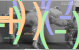
\includegraphics[width=.9\linewidth]{./figures/fig1_landmarks.png}
\caption{\label{fig:landmarks}Video \chng{landmark tracking} and joint angle definitions. White circles mark points of interest (``landmarks''). Movement was always rightwards. Labels show joint angles, defined as shown in the inset: straight joint (parallel segments) corresponds to zero; counter-clockwise \chng{joint} angles are positive. Forelimb \chng{joint} angle was used as a reference for temporal alignment, but did not enter the analysis.}
\end{figure}



The next step is to find the relevant temporal sequences of walking in the continuous videos.
Naturally, the trained network would only extract potentially useful landmark traces for episodes which resembled the training set, i.e. in episodes with a piglet moving perpendicular to the image axis, in lateral aspect and rightward direction.
We automatically extracted \(2597\) of such sequences by filtering for high \chng{landmark position} ``likelihood'' provided by DLC, low noise (i.e. steady landmark movement) and consistent, plausible inter-landmark distances.
We further applied an automatic algorithm to find footfalls and label stride cycles in the candidate episodes (\(4730\) cycles).
This procedure involved a start-end-matching optimization (using Procrustes superimposition, \textit{cf.} Ch. \ref{cpt:fourier_review}) to ensure that strides were indeed cyclical.
To further assess \chng{tracking data} quality, gait variables were automatically extracted.
Definition of these variables was chosen to simplify the automatic procedure, as follows.
Stride distance, frequency, and speed are trivial measures of the animal movement.
Duty factor is available for fore- and hindlimb, and measures the fraction of stride time in which the respective hoof is in ground contact.
Clearance is approximated by quantifying the ratio of flexion of each limb (one minus the quotient of minimum and maximum absolute hip-toe-distance during the stride).
Head and torso angle are the stride-average angles of the snout-ear or withers-croup lines with respect to the coordinate system.
Hindlimb phase measures the time between hind- and forehoof touchdown, divided by the stride cycle duration.
Where applicable, spatiotemporal gait variables were prepared for analysis by converting them to dimensionless values \citep{Hof1996,Alexander1983} using the cumulated distance of landmarks along the snout-to-tailbase line of the animal as reference, extracted as stride average from the \chng{tracked} landmarks.
Only strides with plausible values (i.e. those which lie within the theoretical distribution of each parameter; \(1862\) cycles) where processed.
Manual inspection further boiled down the data set to 897 stride cycles (the others excluded for \chng{tracking} errors, multi-animal confusion, non-walking gait, intermittent or sidewards locomotion, or incompleteness).

Finally, \(368\) of the remaining strides from \(58\) animals were in the youngest age category (\(<10\ h\)) and thus selected for the present analysis, the data table is available online.


\subsection{Data Processing}
\label{sec:orgcb0a26c}

The landmark data provided by DLC was further processed for analysis.
Python code for the whole procedure is available (\nolinkurl{https://git.sr.ht/~falk/piglet_fcas}, Python version 3.10.8 at time of model calculation, \nolinkurl{https://www.python.org}).
First, joint angle profiles (i.e. joint angle values over time) were extracted for all relevant joints and for the total forelimb angle (croup-withers-hoof).
Shoulder, elbow, carpal, hip, stifle, and tarsal were the six joints sufficiently well \chng{tracked} and therefore considered relevant for analysis.
We then applied Fourier Series decomposition in the framework we previously termed Fourier Coefficient Affine Superimposition \citep[FCAS,][and Ch. \ref{cpt:fourier_review}]{Mielke2019}, a flexible procedure which subsumes the following steps.
Joint angle profiles are cyclic, i.e. periodical, and can therefore be transformed to the frequency domain with a Fourier Series decomposition (8 harmonics were deemed sufficient by visual comparison of raw and transformed/retransformed profiles).
In the frequency domain, the affine components (mean, amplitude, phase) of a joint angle profile are easily accessible \citep[\textit{cf.}][and Ch. \ref{cpt:fcas}]{Mielke2019}.
The forelimb angle served as reference to temporally align all cycles in the data set (removal of phase differences between different cycles; forelimb angle was not used further).
Then, mean and amplitude of the joint oscillations were isolated for all joint angles and are categorized as ``dynamic posture'' parameters.
Mean joint angle is the temporal average, whereas amplitude is related to effective range of motion (eROM).
The residual, i.e. differences captured by non-affine Fourier coefficients, can be categorized as ``coordination'' \emph{sensu stricto} (it measures the precise temporal succession of joint configurations).
In our case, there were
\(96\)
variables of coordination (6 \chng{joint} angles, 8 harmonics, real and imaginary) which were submitted to a PCA.
Only the first
\(12\)
coordination components (\(CC\)) were used for statistical analysis, capturing
\(80.2 \%\)
of the variability in coordination.

To summarize, FSD and FCAS served three purposes: (i) temporal alignment of the cyclic traces, (ii) separation of meaningful parameter categories (dynamic posture and coordination), and (iii) preparation for multivariate analysis via PCA.
Basic script code (Python, Matlab and R) to perform FCAS can be found on a dedicated git repository (\url{https://git.sr.ht/\~falk/fcas\_code}).


\bigskip
Information retention is generally a strength of this method.
FCAS and PCA are mathematical transformations, which means that the information content after transformation is theoretically identical to that prior to transformation (theoretically, because only a finite number of harmonics can be used, yet this is of little concern for continuous, smooth joint angle profiles).
The neglected PCs and the residual not captured by 8 harmonics were the only information from kinematics of the given joints to be lost in this procedure, and by definition these contain the least information.
Apart from that, all information present in the raw joint angle profiles enters the analysis.
Though we used a 2D dataset herein, the procedure could be applied equally well to \chng{joint} angles measured from 3D coordinate data \citep{Scott2022}.


Furthermore, all transformations are reversible, hence any analysis outcome can be translated back to kinematics with high accuracy.
Reversibility bares a lot of herein unused potential, for example for interpolating unobserved subject states or for inferring kinematics of fossile species by phylogenetic and morphometric bracketing.
Reversibility can also be of use when presenting raw joint angle profiles and their averages, as follows.
One crucial aspect of the FCAS procedure is temporal alignment of the joint angle profiles in the frequency domain.
In conventional temporal alignment, a single characteristic point in the stride cycle is chosen as a reference, wherein this is only ``characteristic'' for a certain part of one limb (e.g. left hindlimb hoof touchdown).
Temporal alignment to the hindhoof touchdown might cause distinct peaks in the forelimb angle joint profiles to occur at different relative points in the stride cycle (e.g. tarsal joint profiles in Fig. \ref{fig:raw_data}, lower half, green traces).
If profiles show such variable peak positions, then their average will have a wider, less pronounced (i.e. lower amplitude), and potentially unnatural peak.
For illustration, this is analogous to averaging two sine-waves of identical amplitude, but phase shifted: in the worst case, they cancel each other out (as in ``destructive interference'').
The problem is not restricted to pronounced peaks, but generally occurs if the temporal intra-limb coordination varies within a data set.
Using FCAS, it is possible to get a more representative average of the raw traces which has its amplitude conserved, but phase and mean \chng{joint} angle averaged.
This is enabled by transformation to the frequency domain, separation of affine components, removal of phase differences by shifting to average phase, profile averaging, followed by inverse transformation back to the time domain.
Because a set of profiles and phases may be calculated for each \chng{joint} angle individually, and because phase relations can differ between joints, there are the options to align based on one reference angle (e.g. the whole forelimb, as done herein) or minimize all phase differences across all joints.
Chosing the first option herein has implications: when plotting hindlimb joints aligned by a forelimb reference (as in Fig. \ref{fig:raw_data}, lower half), phases still differ, and the ``destructive interference'' problem might hamper averaging.
In such cases it is possible to apply an extra, joint-wise FCAS alignment for the sole purpose of generating meaningful averages.



\subsection{Statistical Modeling}
\label{sec:org7326405}
To summarize, four categories of variables were used for analysis:
\begin{itemize}
\item subject characteristics: age, sex, mass, birth weight category, size
\item spatiotemporal gait variables: distance, frequency, speed, clearance (fore-/hindlimb), duty factor (fore-/hindlimb), head angle, hindlimb phase
\item dynamic posture: mean joint angles and eROM for six joints
\item coordination: the residual after extraction of dynamic posture (see above)
\end{itemize}

Our guiding question for model design is whether a probabilistic, linear model is able to infer subject characteristics (specifically: age, mass, and size) from raw kinematics (expressed as dynamic posture and coordination) and spatiotemporal gait variables (collective variables).
Given the common conception that kinematics are a complex output of an individual motor system, this might be considered an ``inverse'' modeling approach (it is certainly an inversion of the model presented in Ch. \ref{cpt:statistics}).
The present analysis focused on three outcome variables (Fig. \ref{fig:observations}): mass (\(kg\)), size (\emph{arb. units}, from a PCA of marker distances), and age (\(h\)).
Though these outcome variables were specific per individual and recording session, we analyzed them ``per stride'' (i.e. there were multiple strides with identical subject measures on the outcome side).


The model formula is:
\begin{equation} \theta \sim v_{1}\cdot\alpha + v_{s}\cdot\beta_{s} + \sum\limits_{G} v_{g}\cdot\beta_{g} + \sum\limits_{P}  v_{p}\cdot\beta_{p} +  \sum\limits_{C} v_{c}\cdot\beta_{c} + v_{1}\cdot\epsilon \label{eq:model} \end{equation}
Herein, \(\theta\) is either of the outcome subject characteristics, \(\beta\) are slopes associated with the model parameters (\(s\) sex, \(G\) spatiotemporal gait variables, \(P\) dynamic posture, \(C\) coordination), \(v\) are data vectors (e.g. \(v_{1}\) is a vector of ones for the intercept \(\alpha\) and model residual \(\epsilon\), and \(v_{s}\) is a boolean vector coding for subjects of `sex == male`).
The models have a total number of 36 degrees of freedom.
Priors (i.e. \emph{a priori} assigned distributions) for all slopes were Normal distributions with mean and standard deviation corresponding to the mean and two times standard deviation of all observed values of each parameter; logarithmic transform was applied where necessary.
The observable (``likelihood'') prior for \(\theta\) was a Student's T distribution (allows for wider-than-normal tails and robust regression) with a Gamma distributed \(\nu\) (degrees of freedom); \(\epsilon\) was modeled to be a Half Cauchy distribution.
The model was implemented using the Python library ``PyMC'' \citep[version 4.2.2,][]{Salvatier2016}.


To re-emphasize, dynamic posture and coordination together effectively capture all the kinematic information of the stride.
Hence, we train the predictor model with all kinematics, spatiotemporal gait variables, and sex.
Birth weight category (LBW, NBW) is a filter parameter: we split our data set into LBW strides and two NBW subsets (training and validation).
Training is performed by MCMC sampling (`sample` function in PyMC), and a No U-Turn sampler was set to sample with \(32\) chains, each \(2^{14}\) tuning and equally many sampling steps.
All post-hoc model checks confirmed convergence (inspection of traces, \(bfmi>0.94\) for all chains, Gelman-Rubin statistics \(\approx 1\) for all parameters, sufficient effective sample size).
Model comparison was performed (cf. Ch. \ref{cpt:statistics}), iteratively leaving out model parameters or replacing some by meaningful combinations (e.g. duty factor combined for fore- and hindlimb).
However, because we follow an ``all in'' strategy, the results have little instructive value for model construction: we might thus have retained parameters which are numerically unimportant for the NBW-only models.



\begin{figure}[p]
\centering
\includegraphics[width=.9\linewidth]{./figures/histograms_observed.pdf}
\caption{\label{fig:observations}Histogram of observations. Trivially, the LBW group measured the lowest body masses in the data set. This correlated with a lower body size, whereas age is rather uniformly sampled for all study groups. Recordings happened opportunistically within the first ten life hours of the animals, repeated measurements were possible. Number of strides per class are indicated in brackets on the legend. Bar heights are scaled by sample size to show relative value distributions.}
\end{figure}


The data set of \(N = 368\) strides was split into three categories:
(i) the NBW training set as reference with \(N = 294\) strides,
(ii) the NBW validation set (\(N = 35\) strides), which is a random subset of NBW strides, approximately equal in size to
(iii) the LBW test set with \(N = 39\) strides.

The model was thus trained with a set of \(294\) NBW training strides (i).
Inferences (model ``predictions'') were then done per stride, for all observed strides (NBW training, NBW validation, and LBW test), iteratively using the `pymc.sample\_posterior\_predictive` function in PyMC after setting all the data arrays to the actual observed values for one given stride (using `pymc.set\_data`).
The number of predictions usually matches the number of training samples, which means that all posterior information is used to construct the prediction distributions.
We would thus retrieve mass, size, and age predictions (i.e. probabilistic inference) for each stride in the data set, which were then compared to the known, actual mass, size, and age.


All procedures, code, data, and this manuscript are available online (\url{https://git.sr.ht/\~falk/piglet\_fcas}).

\FloatBarrier
\clearpage
\section{Results}
\label{results_22}
The present analysis is centered around a linear model which is designed to infer mass, size, and age (subject characteristics) from an extensive set of kinematic parameters from 2D videos.
The numbers provided by the model sampling are equally extensive, and will only be reported in brief.
The key purpose of the model is posterior predictive sampling of the LBW strides which were left out of the model, and which are analyzed in detail below.


\bigskip

\begin{figure}[p]
\centering
\includegraphics[width=.9\linewidth]{./figures/raw_profile_comparison.pdf}
\caption{\label{fig:raw_data}Joint angle profiles per joint, grouped by birth weight category. A \chng{joint} angle of zero would be a fully extended (i.e. straight) joint. Thick lines represent the average profiles, dashed lines indicate the average of the opposite birth weight group for comparison. Colored, shaded lines show all raw profiles available for the present analysis. Temporal alignment was done based on total forelimb angle (see methods), yet for the shown hindlimb averages (but not for the raw profiles), a separate alignment of the hindlimb was performed.}
\end{figure}

To assess whether there are qualitative differences between the birth weight categories, one can compare the joint angle profiles (i.e. raw, angular kinematics) on which the present analysis was performed (Fig. \ref{fig:raw_data}).
The intra-group variablility clearly exceeds the differences between groups, although it must be emphasized that groups are inhomogeneous (with regard to age, speed, etc.), which might lead to a bias if composition of LBW and NBW data differs.
LBW walk with a more flexed hindlimb posture, as indicated by the parallelly offset average hip, stifle, and tarsal profiles.
Additionally, NBW individuals on average seem to set the shoulder at a more extended \chng{joint} angle.
No differences in coordination are apparent (which would manifest in altered temporal structure of the profiles).
These findings indicate that LBW kinematics are hardly distinguishable from NBW kinematics by qualitative, visual assessment, which is at least in part be due to high variability.



\bigskip

\begin{table}[p]
\caption{\label{tab:modelresults}Detailed Modeling Results. Asterisk (*) indicates slopes for which the credible interval did not include zero. FL: forelimb, HL: hindlimb, dyn.p.: dynamic posture, coord.: coordination, diml.: dimensionless, d.s.: dimensionless stride, eROM: effective range of motion.}
\linespread{1} % Line spacing - Palatino needs more space between lines
\centering
\begin{footnotesize}
\begin{tabular}{rllllll}
 & category & parameter & age (h) & age (log) & size PC1 & mass (kg)\\\empty
\hline
0 & model & intercept & \(+4.86\) & \(+1.68\) & \(-3.25\) & \(+1.38\)\\\empty
1 & subject & female \(\rightarrow\) male & \(+0.05\) & \(+0.00\) & \(-0.38\) * & \(-0.04\)\\\empty
2 & gait & log. FL clearance & \(-0.10\) & \(-0.08\) & \(+0.09\) & \(-0.02\)\\\empty
3 & gait & log. HL clearance & \(+0.94\) * & \(+0.32\) * & \(-0.65\) * & \(-0.15\) *\\\empty
4 & gait & FL duty factor & \(+1.11\) & \(+0.37\) & \(+0.18\) & \(+0.07\)\\\empty
5 & gait & HL duty factor & \(+0.67\) & \(+0.24\) & \(+0.85\) * & \(+0.11\)\\\empty
6 & gait & d.s. distance & \(+1.32\) & \(+0.31\) & \(+0.45\) & \(+0.18\)\\\empty
7 & gait & d.s. frequency & \(+3.12\) & \(+1.43\) & \(+1.62\) & \(+0.15\)\\\empty
8 & gait & diml. speed & \(-1.10\) & \(-0.64\) & \(+0.82\) & \(+0.00\)\\\empty
9 & gait & hindlimb phase & \(-2.04\) & \(-0.56\) & \(-1.98\) & \(+0.05\)\\\empty
10 & gait & head angle & \(+0.26\) & \(+0.14\) & \(+1.44\) * & \(+0.18\)\\\empty
11 & dyn.p. & mean hip angle & \(+2.55\) * & \(+0.59\) * & \(-1.07\) * & \(-0.45\) *\\\empty
12 & dyn.p. & hip eROM & \(+2.64\) & \(+0.94\) & \(-1.34\) & \(-0.52\) *\\\empty
13 & dyn.p. & mean stifle angle & \(+0.67\) & \(+0.10\) & \(-2.01\) * & \(-0.12\)\\\empty
14 & dyn.p. & stifle eROM & \(-1.85\) & \(-0.22\) & \(-1.66\) * & \(-0.13\)\\\empty
15 & dyn.p. & mean tarsal angle & \(-1.18\) & \(-0.59\) & \(+0.44\) & \(+0.23\) *\\\empty
16 & dyn.p. & tarsal eROM & \(-1.92\) & \(-0.88\) * & \(+2.98\) * & \(+0.60\) *\\\empty
17 & dyn.p. & mean shoulder angle & \(+1.06\) & \(+0.07\) & \(+0.47\) & \(+0.06\)\\\empty
18 & dyn.p. & shoulder eROM & \(-0.34\) & \(-0.17\) & \(-0.65\) & \(+0.01\)\\\empty
19 & dyn.p. & mean elbow angle & \(-1.00\) & \(-0.55\) & \(+2.79\) * & \(+0.20\)\\\empty
20 & dyn.p. & elbow eROM & \(+3.22\) & \(+0.96\) & \(+0.11\) & \(-0.30\)\\\empty
21 & dyn.p. & mean carpal angle & \(-2.08\) * & \(-0.98\) * & \(+1.69\) * & \(+0.04\)\\\empty
22 & dyn.p. & carpal eROM & \(-0.24\) & \(+0.21\) & \(-0.84\) & \(+0.16\)\\\empty
23 & coord. & CC1 & \(+0.60\) & \(+0.31\) * & \(+0.10\) & \(-0.05\)\\\empty
24 & coord. & CC2 & \(+0.50\) & \(+0.15\) & \(-0.24\) & \(-0.08\)\\\empty
25 & coord. & CC3 & \(-0.25\) & \(+0.00\) & \(+0.88\) * & \(+0.07\)\\\empty
26 & coord. & CC4 & \(-0.62\) & \(-0.26\) & \(+0.13\) & \(+0.04\)\\\empty
27 & coord. & CC5 & \(-0.84\) & \(-0.25\) & \(-0.16\) & \(+0.04\)\\\empty
28 & coord. & CC6 & \(-1.49\) & \(-0.51\) * & \(-0.10\) & \(+0.07\)\\\empty
29 & coord. & CC7 & \(+0.24\) & \(+0.22\) & \(-0.76\) & \(-0.08\)\\\empty
30 & coord. & CC8 & \(-1.19\) & \(-0.24\) & \(-0.51\) & \(+0.02\)\\\empty
31 & coord. & CC9 & \(-2.96\) * & \(-0.83\) * & \(+0.66\) & \(+0.06\)\\\empty
32 & coord. & CC10 & \(-0.22\) & \(+0.06\) & \(-0.60\) & \(+0.02\)\\\empty
33 & coord. & CC11 & \(-2.05\) * & \(-0.67\) * & \(+0.10\) & \(+0.08\)\\\empty
34 & coord. & CC12 & \(-0.03\) & \(-0.10\) & \(+0.35\) & \(-0.01\)\\\empty
35 & model & \(\epsilon\) & \(\pm 1.81\) & \(\pm 0.56\) & \(\pm 0.98\) & \(\pm 0.20\)\\\empty
\end{tabular}
\end{footnotesize}
\linespread{2} % Line spacing - Palatino needs more space between lines
\end{table}



A quantitative comparison of variable kinematic measurements can be achieved with probabilistic linear models.
For the purpose of predictive sampling, we train models to describe the interrelations of kinematic parameters and subject characteristics in NBW piglets.
The outcome of MCMC sampling of a linear model are value distributions for slopes, which in our case indicated how certain kinematic parameters are associated with a change in mass, size, and age (Tab. \ref{tab:modelresults}).
Of the gait- or coordination parameters, only hindlimb clearance was correlated with differences in animal mass.
Mass was also associated with changes in the dynamic posture of the hip and tarsal.
For size, the model inferred associations with head angle, hindlimb duty factor and clearance, and one coordination component (CC3), as well as changes in the fore- and hindlimb posture and an effect of sex.
Finally, age was associated with an increase in forelimb clearance, potential changes at the stifle and carpal, and several coordination components (CC9, CC11).
Some eROM slope distributions for age were high in average magnitude, but variable (the ``credible interval'' contained zero).
These model results provide detailed insight into parameter interrelations in the present data set and indicate which of the parameters are the relevent ones to infer a given subject attribute in predictive sampling.



\bigskip

Performing in-sample and out-of-sample predictive inference with the models trained on NBW strides elucidated if and how left-out strides differed from NBW model expectation (Fig. \ref{fig:predictions}).
Note that, to capture variance (i.e. uncertainty in the prediction), each stride was sampled repeatedly.

\begin{figure}[p]
\centering
\includegraphics[width=.9\linewidth]{./figures/histograms_prediction_comparison.pdf}
\caption{\label{fig:predictions}Predictive sampling of subject characteristics. For all included subject characteristics, models which were trained on NBW strides correctly inferred the training data (gray) and values from the validation set (blue). In contrast, the same models wrongly inferred the characteristics of LBW subjects (orange). The \(x\)-axes show the difference (\(\Delta\)) between actual and predicted values per prediction. To facilitate comparison, histogram heights are again normalized per category.}
\end{figure}


Out-of-sample inferences for the \emph{NBW validation set} matched those of in-sample NBW inference in terms of average values and standard deviation for all modeled outcome variables, which confirms that inference of subject characteristics from kinematics is possible.
In contrast, inferences for the \emph{test set} of LBW strides did not match those of the NBW training set.
Low birth weight animals were inferred to be on average \(0.44 kg\) heavier than actual, and their size was overestimated (\(+1.71\)
units).
Both faults matched the actual differences in magnitude (\emph{cf.} methods, Fig. \ref{fig:observations}).
In contrast, the age inference for the low birth weight subjects were not normally distributed: most ages were correctly inferred from stride-wise kinematics, but ages for some strides were underestimated.
The underestimation of those strides quantified to just below five hours.

In summary, the NBW-trained model ``guesses'' the size and mass of the animals producing LBW strides to be ``normal'' (although they are not), which indicates that these defining features of LBW do not reflect in altered kinematics.
However, age inference is non-normal, i.e. some strides are classified as typical for animals of younger than actual age.


\begin{change}
These findings are based on an analysis which uses the statistical model of one subset of the data for predictive inference on another subset, which is a strategy that demands justification.
\begin{itemize}
\item Is the model actually \textit{capable} of finding differences?
\item Under which circumstances will group differences arise?
\item Is there a bias in the modeling procedure, for example to not find all differences?
\begin{itemize}
Answering these questions requires a rather technical analysis of the model outcome.

One important constraint is that the model is linear, i.e. of the form
\[y = a + b_1 \cdot x_1 + b_2 \cdot x_2 + \ldots + b_m \cdot x_m + \epsilon = a + \sum\limits_k b_k \cdot x_k + \epsilon\]

Herein, \(y\) is one of the outcome variables (observed; age, size, or mass), \(a\) is the intercept, \(b_i\) are the slopes, \(x_i\) are the different input parameters (observed; spatiotemporal gait variables, dynamic posture, and coordination measures), and finally \(\epsilon\) is the model residual (unexplained variation).
As I have demonstrated \href{http://mielke-bio.info/falk/posts/33.linearmodels}{elsewhere} \citep{Mielke2024lm}, there are some conditions which are necessary (but not sufficient by themselves) to find a difference.
If there is a...
\begin{enumearate}
\item significant difference between the study groups in the distributions of input variables
\item high enough slope magnitude (``steepness'')
\item small enough model complexity/size, i.e. limited number of (other) slopes
\item low residual variation or noise
\item sufficient sample size
\begin{enumearate}

... then we can find differences as in the example of age, above.
In case one of these conditions is not met, a difference between the study groups might be obscured (yet note that there is a continuum, and effects may cancel).
Note that, from theoretical considerations alone, this situation is biased.
Differences in out-of-sample prediction (e.g. in case of the age model) must have passed the criteria above, and are therefore robust.
On the other hand, \textit{"the absence of evidence is not the evidence of absence"}: if for example the sample size is low, or the residual variation is high, the model's prediction might have missed an actual effect.
This situation is somewhat analogous to classical hypothesis testing.

\begin{figure}[p!]
\centering
\includegraphics[width=16cm]{./figures/input_distribution_differences.pdf}
\caption{\label{fig:input_distributions}Observed model parameter input distributions. Observations are indicated for each model parameter (rows) by tick marks for the two study groups (NBW: gray, LBW: orange). Values were standardized (mean-centered and scaled by standard deviation). Significance between the distributions (indicated by asterisk) was determined by a two-sample ranksum test.}
\end{figure}

\begin{figure}[p!]
\centering
\includegraphics[width=16cm]{./figures/output_effectsize.pdf}
\caption{\label{fig:output_effects}Effects of each input parameter on the model output. Effect size is calculated as the data range (difference between \(2.5\%\) and \(97.5\%\) data quantiles) multiplied by the slope distributions (from model sampling). Effect magnitude is visualized by red shading, effects which are different from zero (\(95\%\) HDI) are also indicated by an asterisk. Residual is determined as the difference of the actual parameter observation and the model result.}
\end{figure}


The available modeling framework enables some extra insights on why the prediction appeared as it did.
Firstly, we can compare the input distributions (point 1) of the observational groups (Fig. \ref{fig:input_distributions}), to identify those model parameters which acutally influence the predictions.
Secondly, we can calculate the absolute effect of each parameter onto the predicted outcome (slope magnitude, point 2), by multiplying the parameter magnitude with the according slope (Fig. \ref{fig:output_effects}; this works because \(\Delta y \sim b_i \cdot \Delta x_i\)).
Thirdly, we can quantify the model residual (point 4; Fig. \ref{output_effects}).
The other points above (model complexity and sample size) are fixed in our application, and could have an influence which here remains undetermined.

For the \textbf{age model}, we observe a low residual variance, and there are two parameters which are significantly different between NBW / LBW \textit{and} have a high slope (those are hindlimb clearance and hip angle).
Notably, there is hardly any difference in the observed coordination parameters.
For the model of \textbf{body mass}, the same parameters seem to have relevant slopes, yet the model residual is much higher and will likely prohibit conclusive differences in the probabilistic prediction.
Other slopes seem to have significant effect in the NBW group (hip and tarsal eROM), yet the input distributions (i.e. NBW and LBW observations) do not differ, and so their effect is irrelevant for prediction of mass.
For the \textbf{size model}, we find some slopes with a negative effect on the output (hindlimb clearance, head angle, hip angle), yet others with a positive effect (knee angle, tarsal eROM) possibly cancel this out for the overall prediction.
This model also contains significant slopes with nonetheless no difference in the input distribution.
We also compared the relative widths of effect size distributions, and found that "dimensionless (relative) speed" is most variable among trials: all animals use a variety of speeds, and this can not be systematically associated with age, size, or mass.
It must be re-iterated that "significance" in these analyses merely provides a hint to guide the eye: the combination of a minor (non-significant) difference in an input parameter with a notable, only "almost-significant" effect size might still affect the probabilistic prediction.
Finally, the input distributions (Fig. \ref{fig:input_distributions}) are insightful by themselves for NBW / LBW comparison.
We observe most differences in spatiotemporals (predominantly hindlimb-related), as well as in measures of dynamic posture and range of motion.
However, there are few significant effects of coordination parameters, and the remaining ones are canceled out by a lack of difference in the observed coordination of LBW and NBW.


To summarize, we show that a detailed inspection of on the one hand the observed model input parameters, and on the other hand the effect "lever" of each parameter slope, warrants some caution about non-different predictions (as in the models of size and mass).
In those models, we cannot rule out that a larger sample size or an adjusted, potentially more selective model design might elucidate quantitative NBW/LBW differences.
On the other hand, inspection of the predictive age model confirms that finding differences by out-of-sample prediction is possible, and we could even relate those findings to specific model parameters.

\end{change}





\bigskip


\begin{table}[p]
\caption{\label{tab:prediction}Age inference per LBW animal (compared to NBW average, last row). \(\Delta\): ``inferred - actual'' difference. Underestimation is defined as \(\Delta < 0\), ``count'': per stride, ``rate'': per predictive sample. \(h\): hours, \(std\): standard deviation.}
\centering
\begin{tabular}{|l|c|c|c|c|c|c|}
\hline
  \textbf{piglet} & \textbf{age} & \textbf{strides} & \multicolumn{2}{c|}{\textbf{underestimation}} & \textbf{pred. mean} \(\Delta\) & \textbf{pred. std}
  \\\hline \empty & h &  & count & ratio & h & h\\\empty
\hline \hline
b23 & 2.0 & 6 & 0 & 0.29 & 1.13 & 2.00\\\empty
b15 & 2.9 & 5 & 0 & 0.37 & 0.68 & 1.96\\\empty
b76 & 3.1 & 4 & 0 & 0.39 & 0.57 & 2.01\\\empty
b74 & 4.2 & 7 & 1 & 0.40 & 0.52 & 1.97\\\empty
1794.5 & 5.6 & 5 & 5 & 0.90 & -2.57 & 1.99\\\empty
b58 & 7.8 & 3 & 3 & 0.91 & -2.85 & 2.00\\\empty
b19v2 & 9.8 & 1 & 1 & 1.00 & -6.14 & 1.99\\\empty
b56 & 9.9 & 8 & 8 & 0.99 & -4.58 & 1.96\\\empty
\hline
<all NBW> & <3.8> & 329 & 158 & 0.49 & -0.03 & 1.95\\\empty
\hline
\end{tabular}
\end{table}


To find out whether the offset age inference was related to certain individuals, or certain strides from different individuals, we grouped the inferences per stride or subject and calculated the chance of over- or underestimating age.
Of the
\(8\)
low birth weight subjects who contributed
\(39\)
strides,
\(4\)
individuals were consistently underestimated (Tab. \ref{tab:prediction}).
Consistently means that more than \(75 \%\) of all predictive samples were below actual age, and that the ages for a majority of strides were on average underestimated.
The magnitude of underestimation was between two and five hours.
Curiously, those were the individuals recorded at a slightly higher age (\(> 5\) hours).
Overestimation in the other four LBW individuals was also consistent, but less so (less extreme underestimation rate, mean \(\Delta < 2\ h\)).
Standard deviation of the estimates did not vary across individuals or birth weight categories.

We conclude that underestimation of age is consistent over multiple strides of the same individual, and thus individual-specific.

\FloatBarrier
\clearpage
\section{Discussion}
\label{discussion_22}

Birth weight variability in piglets is considerable.
The average birth weight of a new born piglet in our data set is just above a kilo, yet the span within a litter is typically above \(800\ g\).
Size ranges are accordingly high.
Low birth weight is often associated with low vitality \citep{Baxter2008,Hales2013,Muns2013}, and this supposedly correlates with deficient locomotion.
Previous studies reported behavioral, physiological, and other differences for piglets of low body mass which could affect locomotion \citep{Quiniou2002,Muns2013,VandenHole2018b,Alvarenga2013,VandenHole2018,Roelofs2019}.
One might therefore anticipate differences in how these newborn animals move their more or less heavy bodies, which is the immediate outcome of motor control.
Top-down, direct, visual assessment could justify the hypothesis that LBW walking kinematics are somehow different from ``normal'' \citep{DEath2012}.
Yet that is (i) hard to assess due to high behavioral variability and (ii) trivially expected given the adaptation to different physical properties of their body: gravitational force is a predominant constraint of locomotion, and it simply scales with animal weight \citep{Aerts2023}.
The overarching question is whether low or critically low birth weight can be quantitatively associated with a deficit in locomotion.


However, we observe little qualitative difference in LBW and NBW kinematics (Fig. \ref{fig:raw_data}).
There is a small difference when averaging hindlimb posture, which might be trivially explained by inhomogeneous group composition (but see below).
This is further supported by the fact that our models were unable to correctly retro-infer either mass or size from blindly provided kinematic parameters, including coordination.
Strides from LBW animals were estimated to come from an animal with a ``normal'' mass and size (Fig. \ref{fig:predictions}).
This suggests that low body mass or small size can not be causal for altered 2D kinematics, and it raises doubts whether there are any deficits in coordination and control.
Within the range of kinematic variability, we observe LBW animals perfectly \emph{capable} of normal posture, coordination, and overall stride results (collective variables).
Note that this does not rule out problems of balance, stability, or endurance.


We do see differences for LBW compared to NBW recordings, nonetheless.
First, a difference in sample size.
There are much fewer valid LBW strides in our data set: only \(39\) of \(368\) observations are LBW.
This could be interpreted as evidence for a lower capacity  of LBW to produce normal locomotion (i.e. they succeed in this locomotor task less frequently, despite equal potential).
Yet there are proximal, trivial explanations: based on conventions, the \(10 \%\) lower quantile of birth weights in a litter is considered LBW, and there is a hard cap of \(800\ g\).
The resulting share is equal in our training set for video \chng{tracking}, and in the final data set, because of pseudo-random, opportunistic sampling on-site (i.e. recording work was permanent, yet determined by farrowing and feeding of the subjects).
The minority of LBW training videos might lead to an under-learning of those animals, reduced \chng{landmark tracking} quality and therefore an exclusion bias for ``non-normal'' individuals.
Though it seems unlikely, we cannot rule out reduced locomotor endurance in LBWs, because the present data set is unsuited to count the occurrence of locomotor behavior.
On the other hand, the strict stride filtering criteria for ``good'' kinematics may have involuntarily filtered out deficient individuals.
Our conclusion that low birth weight individuals are non-deficient is strictly tied to the definition of the low birth weight category, which is herein based on weight criteria and did not regard phenotypical indicators of intra-uterine growth restriction \citep[which we did not record, \textit{cf.}][]{Amdi2013}.


A second difference of LBW locomotion is that the age is underestimated for strides of some, but not all individuals.
Prediction is consistent per individual, although no subject characteristics except sex entered the model (``blind'' inference).
This supports the hypothesis that locomotor development is sometimes delayed in LBWs.
Delayed development does not necessarily corroborate the hypothesis of locomotor deficiency in LBW: we would expect truly deficient strides to be substantially different from the data trained to the model, making it ``unpredictable'' (i.e. higher variance of posterior samples).
Instead, the predictions are consistent for repeated measures of an individual, without notable increase in variance.
For the affected subjects, we can even quantify a delay of less than five hours, which could nevertheless be critical given the rapid maturation of locomotor behavior in this species \citep{VandenHole2017} and the importance of postnatal competition \citep{Litten2003}.


Note however that the causality might be inverse.
We measured age underestimation only in the case of the individuals which were recorded late within our sampling time frame (age \(> 5\ h\), Tab. \ref{tab:prediction}).
This is consistent with prior evidence that energy reserves are depleted after birth (normal locomotion) but not replenished after four hours in the case of LBW \citep{LeDividich2017,VandenHole2019}.
Assuming that this is the case, i.e. energy reserves are depleted, we would expect two effects: (i) the animal might succeed in the locomotor task less frequently (not quantified, see above), and (ii) the kinematics might be altered, which we observed.
The present model was trained from NBW data and thereby tuned to kinematic development from animals with normal energy levels (therefore it can correctly infer age from kinematics in NBW).
That same model quantifies the potentially energy-deficient animals as younger.
It might be that energy deficiency coincidentally causes effects which are exactly opposite to the changes that piglet kinematics undergo in normal development.
However, the more likely explanation is an actual delay or a temporary halt in development.
Failure of the LBW to compete in the first hours are sufficient to explain reduced intake \citep{Amdi2013}, the absolute size and mass difference alone might be crucial, and an immediate question which we cannot address with the present data set is whether and how (fast, likely) animals would recover from the delay.
Alternatively, there might be a technical artifact in probabilistic sampling \citep["shrinkage", \textit{cf.}][]{Gelman2013} which caused the underestimation of ``above average age'' individuals.
Yet this is an unlikely explanation, given that shrinkage would apply equally to NBWs, and inversely to the opposite, younger subjects.
Finally, with only eight LBW individuals, we cannot exclude coincidence in which individuals are affected.

Neither of these technical explanations puts doubt on the clarity of the initial finding: a subset of the low birth weight individuals produced locomotor behavior which is quantitatively similar to that of younger individuals.



A corollary question is which patterns in the kinematic variables cause the different age inferences.
We report high magnitude (but also highly variable, i.e. ``non-significant'') slopes inferred from the age model (Tab. \ref{tab:modelresults}).
Note that these slopes solely reflect effects within the NBW data subset.
We also observed slight differences in the average hindlimb dynamic posture (Fig. \ref{fig:raw_data}).
In fact, a more flexed hindlimb is typical for the youngest animals of both birth weight categories.
We emphasized potential differences in group composition to explain that (e.g. sex effect in the ``size'' model), and different age per group might be a proximal explanation for the non-normal age inference in LBW.
However, the average age of LBW animals (\(5.3 h\)) in our data set is nominally above that of NBW (\(3.8 h\)), which is a discrepancy with the age underestimation.
Yet if we assume that the hypothesis of delayed locomotor development is correct, the nominal age would be misleading, and LBW effectively behave similar to younger animals.
This can explain the apparent discrepancy in age group composition and age predictions from kinematics.
It also suggests that dynamic posture might be the major proxy for perinatal maturation, though many other parameters also entered the probabilistic model and influenced the model outcome.


\bigskip

The findings discussed above are enabled by ``inverse'' modeling of subject characteristics as a function of kinematic parameters, using probabilistic models.
The models do reveal various parameter associations, yet the top down (repeated) testing with the chosen model structure complicates drawing definite conclusions \citep[e.g. we observed a sex effect on size, but opposite of what other studies have reported,][we conclude males in our study were just smaller by chance]{Baxter2012}.
Instead, the demonstrated predictive modeling strategy \citep{Shmueli2010} leverages the potential of probabilistic models to perform out-of-sample prediction (via separation of the LBW test group).
Non-probabilistic modeling could equally serve to predict values, but it cannot generate parameter distributions (as in the bimodal age predictions, Fig. \ref{fig:predictions}).
Our probabilistic models implicitly regard ``non-significant'' parameter slopes, which are usually neglected in standard hypothesis testing (such as the high magnitude, highly variable joint ROM quantities, which might nevertheless have relevance for age prediction in case they are correlated and add up).
The data transformations and predictive modeling strategy we applied herein hold further potential for inferring kinematics, for example by morphometric bracketing of extinct taxa.
For that purpose, one would train a model to infer dynamic posture and coordination from a given range of morphometrics, predict samples for specific morphometrics in that range, and convert the samples back to (3D) joint angle profiles which could be animated.


There is a conceptual hierarchy, but no clear causality, with regard to modeling parameter dependencies in quantitative studies of locomotion.
For example, animals might increase the hip angle (posture) and the temporal pattern in the joint angle profiles (coordination) to reach higher speeds (spatiotemporal gait variables), but the speed they reach might depend on age (i.e. maturation, a subject parameter).
But maturation and age might also influence the speed without changing dynamic posture or coordination, simply because the animal grows and increases strength.
Age might also affect dynamic posture and coordination directly, for example if dimensionless speed stays constant but clearance changes with age.
Reducing clearance can increase speed (less unnecessary hoof lifting) or reduce it (higher duty factor), which can be distinguished by the other parameters.
This complex interrelation of spatiotemporal quantities complicates the intuitive modeling strategy, which involves using subject characteristics as a factor to predict a multivariate block of spatiotemporal gait variables and kinematics.
In our experience, model residuals in such models are high, multiple testing can yield putatively coincidental significances, cross-dependencies within the multivariate data set might be underestimated, and sample size requirements are high.
And even under ideal circumstances: chances are that such models would yield \emph{some} age effect, even with random data.

\medskip
In contrast, the strategy applied herein is related to the question: ``given the complete kinematic output of a behavior, can we infer subject characteristics of the animal producing it?''
We used probabilistic, predictive models, which are able to capture intrinsic variability of the process, and addressed specific categorical questions (NBW/LBW differences) by out-of-sample predictions.
We demonstrated that, in the first ten hours of piglet life, (1) kinematics seem to be indifferent to low body mass and size, and (2) locomotion of some LBW individuals could be explained by a delay in locomotor maturation which is initiated \emph{post partum}.




\FloatBarrier
\clearpage
\section{Acknowledgements}
\label{sec:org2d8bfbc}
The author would like to thank Miriam Ayuso for organizing and participating in the recording sessions, as well as Laura Buyssens, Georgios Petrellis, Gunther Vrolix, Charlotte Vanden Hole, Denise Vogel and all students who joined for help during recordings.
Maja Mielke provided valuable comments on the manuscript text.


\FloatBarrier
\clearpage
% \bibliographystyle{apalike}
% \bibliography{literature.bib}
